\newpage
\begin{flushright}
	\textit{Research is what I am doing when I do not know what I am doing}.\\
    \textbf{-- Wernher von Braun}
\end{flushright}

\prefaceChapterTitle{Acknowledgments}{19}{24}{35}

\normalsize
\libertineNormal

% \lipsum[1-6]

% On a technical level, these last three years have considerably contributed to improving as a researcher. The work carried out has led to important results that have been published in top journals and conferences from the Remote Sensing field, while others are still under review. In addition, I have had the pleasure of contributing to other colleagues' work, and despite those publications not fitting in this dissertation, they have greatly contributed to broadening my knowledge of Computer Graphics in other fields which are not my main area of expertise. 

\noindent Con esta tesis culminan tres duros años de trabajo con demasiadas emociones encontradas. Tres años de desafíos, alegría, frustración y aprendizaje en los que muchas personas han aportado su granito de arena para que todo esto fuera posible. 
% He descubierto una infinidad de trabajos y líneas de investigación que de otra forma no hubiera sido posible, e igualmente, ha servido para despertar mi interés por la ciencia. 

\noindent En primer lugar, me gustaría expresar mi más sincera gratitud a mis directores de tesis, Francisco Feito y Carlos Ogayar, por darme la oportunidad de investigar y trabajar con ellos. Jamás hubiera pensado que podría investigar, o que me gustaría, y lo que no me imagino en este momento es no continuar haciéndolo. Muchas gracias por confiar en mí y permitirme llevar a cabo trabajos que han derivado en tantos éxitos. También me gustaría agradecer a aquellos profesores que, con su labor docente, despertaron en mí el interés por la informática gráfica, especialmente a Francisco Conde. 

\noindent Por otro lado, también quiero agradecer a mis padres y mi hermano por apoyarme durante todo este camino y por todas las oportunidades que me han dado. Todas las emociones que he experimentado en estos tres años, y en especial las emociones negativas, también las han sufrido ellos.

\noindent Igualmente, quiero transmitir mi gratitud a todos los compañeros de departamento y del grupo de investigación de Informática Gráfica y Geomática que me han acompañado en esta aventura: Rafael, Juanma, Ángel Luis, Lidia, Isabel, y en especial, me gustaría agradecer a Roberto por sus valiosos consejos en estos últimos meses. 

\noindent Muchas gracias a todos los compañeros del A3-102, A3-103 y A3-155 por ayudarme a dejar a un lado mis problemas durante media hora de charla y café, y en especial a Dani, Alicia, Jesús, David, María, Inma, Gema, José Antonio, José Negrillo, José Luis Cárdenas, Alejandro, Juan Carlos y Adrián. Igualmente, me gustaría agradecer a mis compañeros de laboratorio, Diego, Andressa, Álvaro, Wen y Bruno, por aguantarme cada día, y especialmente a Diego por hacer más amenas demasiadas tardes de trabajo. 

\noindent Finalmente, me gustaría transmitir mi agradecimiento a Joaquim por permitirme realizar mi estancia de investigación en la Universidad de Trás-os Montes e Alto Douro, en Vila Real, donde me sentí como si llevara toda una vida. 

\vspace{50mm} 

\noindent Esta tesis ha sido financiada por el Ministerio de Ciencia, Innovación y Universidades mediante un contrato predoctoral FPU (FPU19/00100) y una ayuda de movilidad dentro de este mismo programa (EST22/00350).  

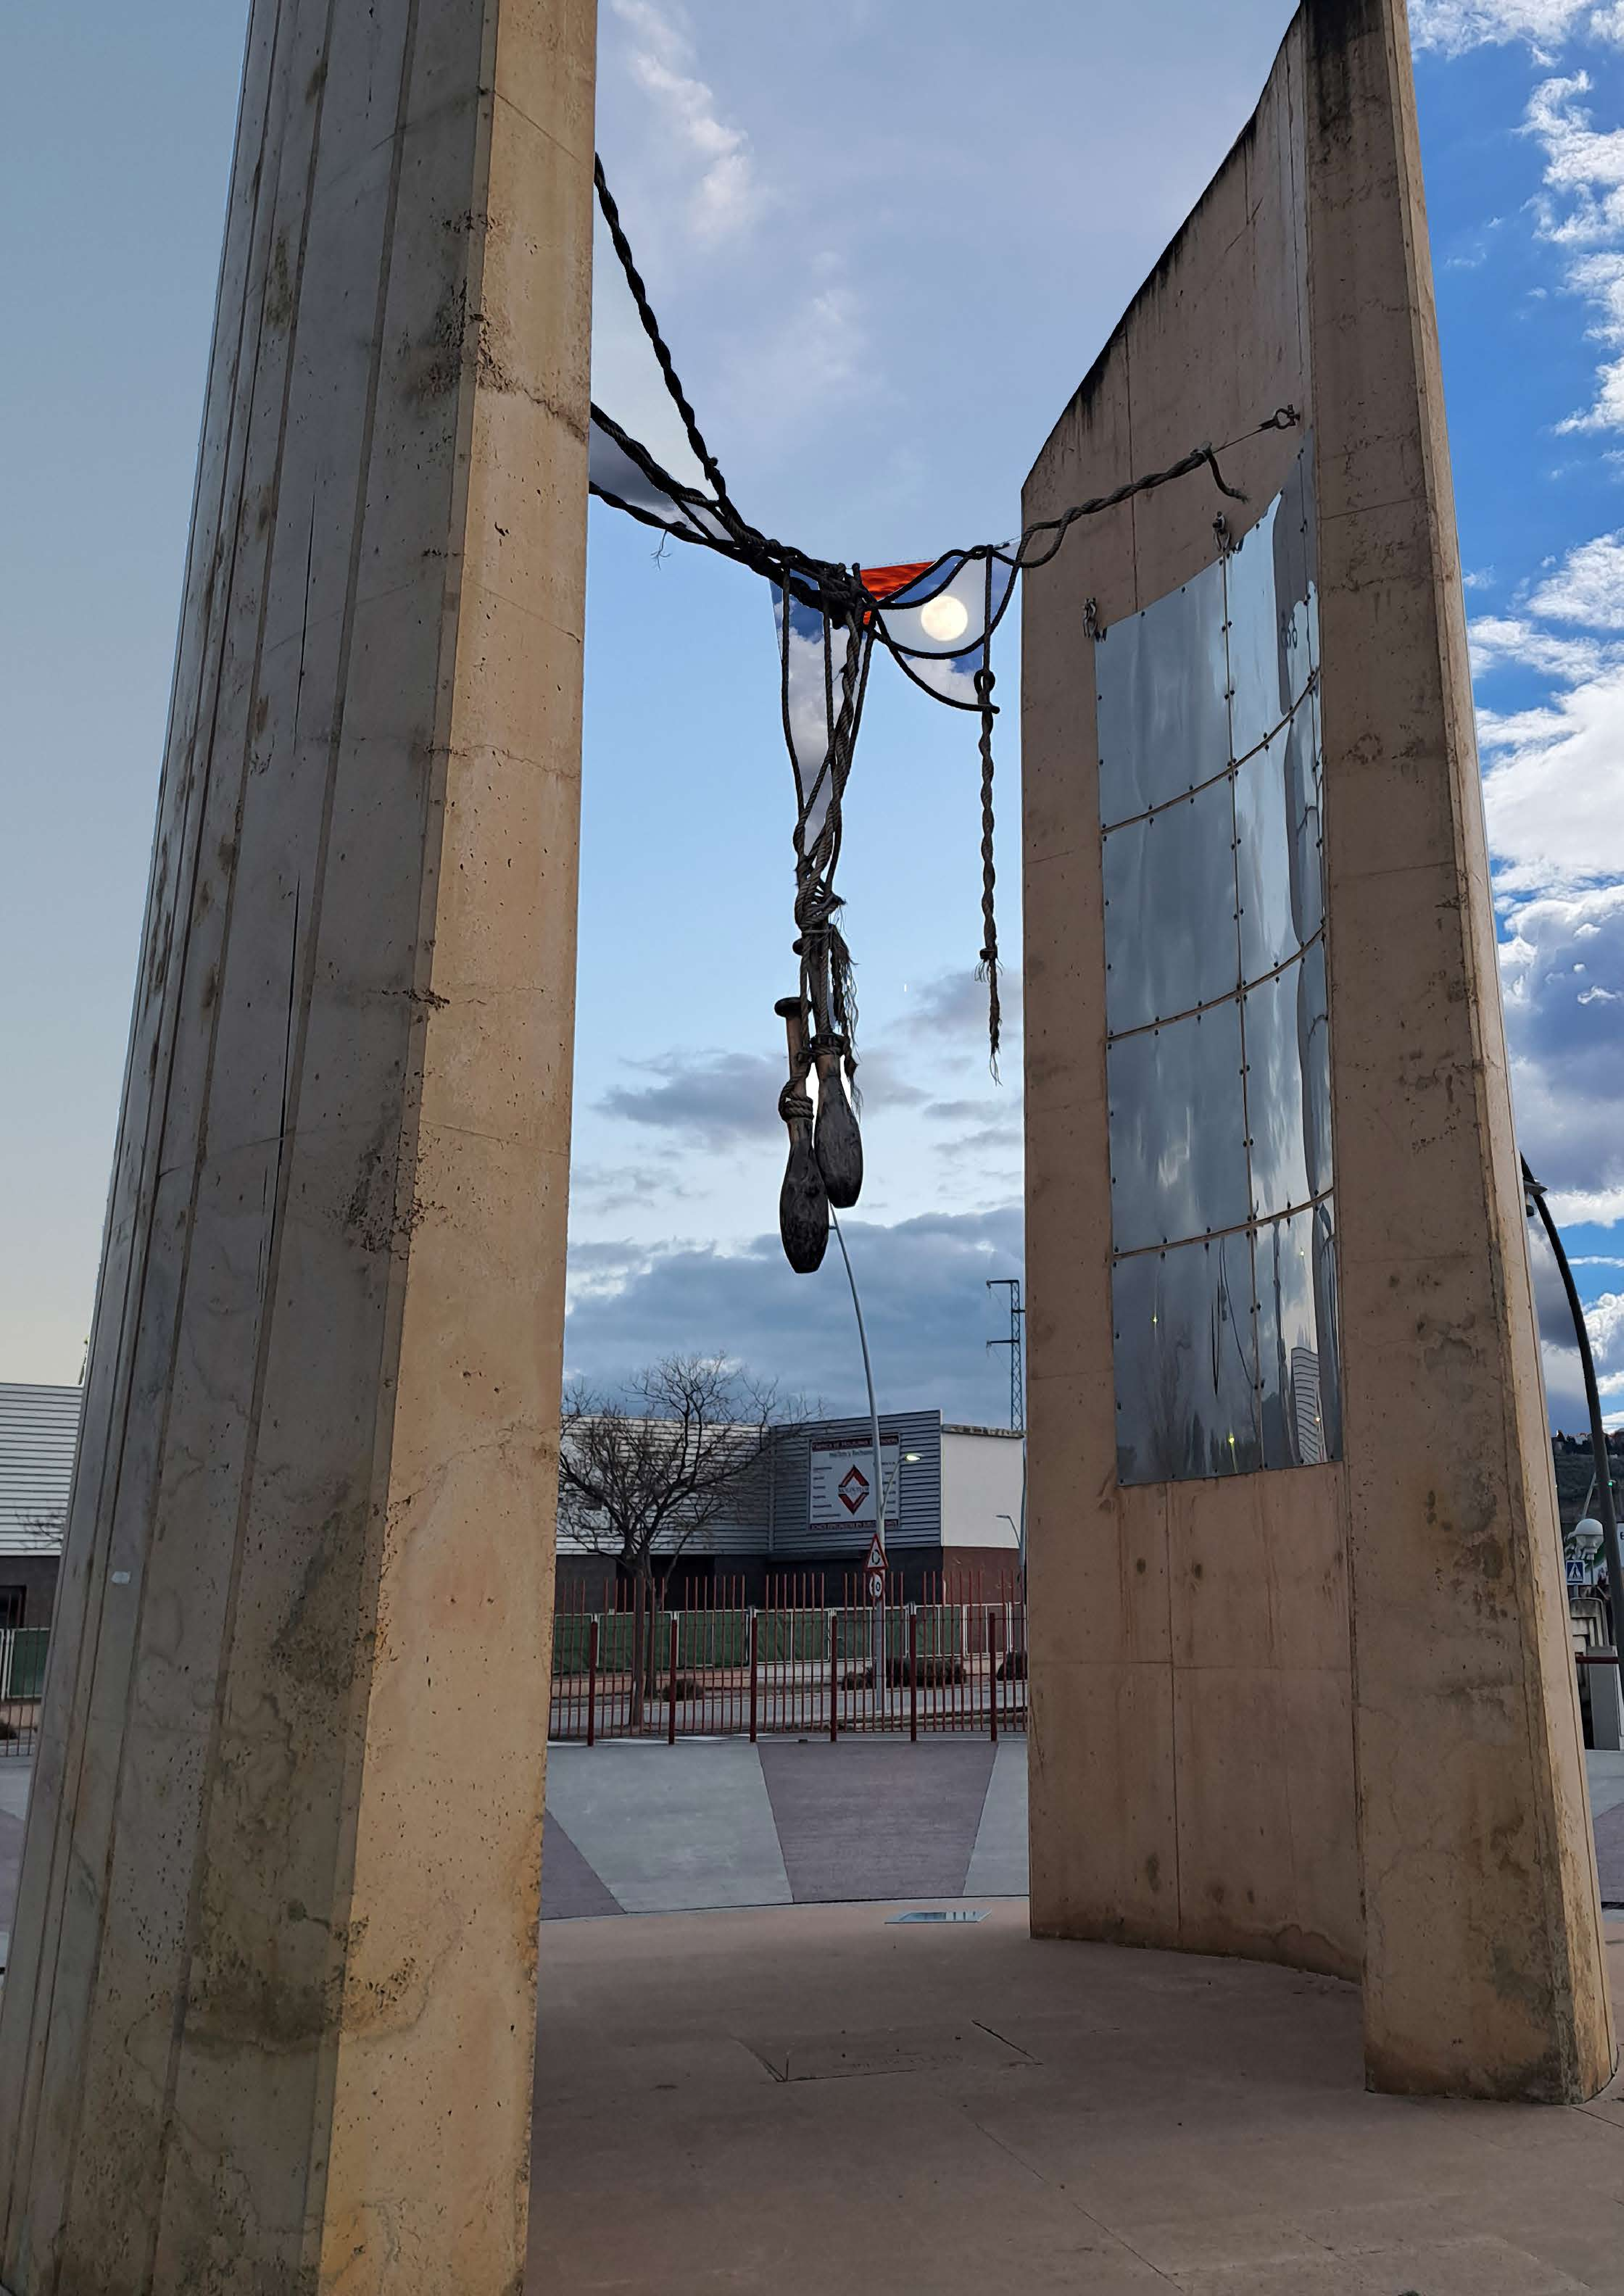
\includepdf[pages=-]{figs/acknowledgments/cover.pdf}